\documentclass[11pt]{article}

% This is a package for drawing figures
% it is a part of standard latex 2e distribution
\usepackage{tikz}
\usetikzlibrary{shapes}
\usepackage{fullpage}


\usepackage{palatino}
\RequirePackage{ifthen}
\usepackage{latexsym}
\RequirePackage{amsmath}
\RequirePackage{amsthm}
\RequirePackage{amssymb}
\RequirePackage{xspace}
\RequirePackage{graphics}
\usepackage{xcolor}




\RequirePackage{textcomp}
\usepackage{keyval}
%\usepackage{listings}
\usepackage{xspace}
\usepackage{mathrsfs,paralist, amsmath,amssymb,url,listings,mathrsfs}
%\usepackage{pvs}
%\usepackage{supertabular,alltt,latexsym}
%\usepackage{multicol,multirow,epsfig}
%\usepackage[dvips, usenames]{color}
\usepackage{framed}
\usepackage{lipsum}
%\usepackage[dvipsnames]{color}

% copyright notice


\definecolor{reddish}{rgb}{1,.8,0.8}
\definecolor{blueish}{rgb}{0.8,.8,1}
\definecolor{greenish}{rgb}{.8,1,0.8}
\definecolor{yellowish}{rgb}{1,1,.20}


\usepackage[pdftex]{hyperref}
\hypersetup{
	pdftitle={Lecture notes for Modeling and Verification of Real-time and Hybrid Systems},
	pdfauthor={Sayan Mitra},
	colorlinks=true,
	citecolor={blue},
	linkcolor = {blue},
	pagecolor={blue},
	backref={true},
	bookmarks=true,
	bookmarksopen=false,
	bookmarksnumbered=true
}

%\newcommand{\remove}[1]{}
\newcommand{\nicole}[1]{\textcolor{red}{#1}}

\newcommand{\handout}[6]{
	\noindent
	\begin{center}
		\framebox{
			\vbox{
				\hbox to 5.78in { {\bf ECE/CS 584: Embedded and cyberphysical system  verification } \hfill #2 }
				\vspace{4mm}
				\hbox to 5.78in { {\Large \hfill #5  \hfill} }
				\vspace{2mm}
				\hbox to 5.78in { {\Large \hfill #6  \hfill} }
				\vspace{2mm}
				\hbox to 5.78in { {\em #3 \hfill #4} }
			}
		}
	\end{center}
	\vspace*{4mm}
}

\newcommand{\smallheader}[5]{
	\noindent
	\begin{center}
		\framebox{
			\vbox{
				\hbox to 5.78in { {\bf ECE/CS 584: Embedded and cyberphysical system  verification  } \hfill #2 }
				\vspace{2mm}
				\hbox to 5.78in { {\em #3 \hfill #4} }
				\vspace{2mm}
				\hbox to 5.78in { {\em \hfill #5} }
			}
		}
	\end{center}
	\vspace*{4mm}
}

\newcommand{\lecture}[4]{\handout{#1}{#2}{#3}{Scribe: #4}{Lecture #1}}

\newcommand{\homework}[2]{\smallheader{#1}{Fall 2019}{Homework #1}\vspace{5mm}
	{#2}
}

\newcommand{\solution}[2]{\smallheader{#1}{Fall 2017}{Solutions for Homework #1}{#2}}


\newcommand{\interestingfact}[1]{
	\noindent
	\begin{center}
		\colorbox{yellowish}{
			\parbox{11.5cm}{{\bf Factoid.} #1}
		}
	\end{center}
	\vspace*{4mm}
}
%\definecolor{MyGray}{rgb}{0.96,0.97,0.98}
\makeatletter\newenvironment{color1box}{%
	\begin{lrbox}{\@tempboxa}\begin{minipage}{\columnwidth}}{\end{minipage}\end{lrbox}%
	\colorbox{reddish}{\usebox{\@tempboxa}}
}\makeatother


\makeatletter\newenvironment{color3box}{%
	\begin{lrbox}{\@tempboxa}\begin{minipage}{\columnwidth}}{\end{minipage}\end{lrbox}%
	\colorbox{blueish}{\usebox{\@tempboxa}}
}\makeatother

% 1-inch margins, from fullpage.sty by H.Partl, Version 2, Dec. 15, 1988.
\topmargin 0pt
\advance \topmargin by -\headheight
\advance \topmargin by -\headsep
\textheight 8.9in
\oddsidemargin 0pt
\evensidemargin \oddsidemargin
\marginparwidth 0.5in
\textwidth 6.5in

\parindent 0in
\parskip 1.5ex
%\renewcommand{\baselinestretch}{1.25}

\begin{document}

\smallheader{3 on --- Due on November $14^{th}$}{Fall 2019}{Dawei Sun, daweis2}{Homework 5: Progress verification}{Due Dec $5^{th}$}

%\homework{5 Theorem proving and stability--- Due on November $29^{th}$, 2019}{Your name}


\begin{quote}
	{\em Typeset your solutions using \LaTeX\, zip your writeup (.pdf) and code in a single file called \texttt{nedid-584-F19.zip} and upload this file through Compass.}
\end{quote}





\paragraph{Problem 2 (25 points).}
In the following hybrid automaton (switched system) $\A$,
$a_1, a_2, c_1 \in \plreals$ and $b_1, b_2 \in \reals$
are constant parameters of the model.

\begin{figure}[h!]
	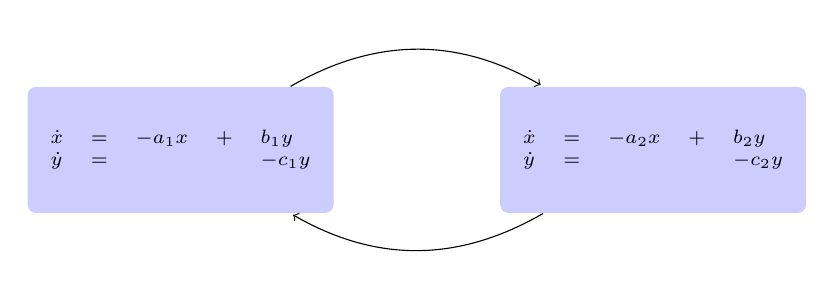
\begin{tikzpicture}
	\tikzstyle{every node}=[font=\scriptsize, rounded corners=3pt, fill=blue!20, font=\scriptsize, minimum size = 1.6cm]
	\draw (-3,3) node (p1) {$\begin{array}{lllll} \dot{x} & = & -a_1 x &+& b_1 y \\ \dot{y} & = &  & & - c_1 y \end{array}$};
	\draw (3,3) node (p2) {$\begin{array}{lllll} \dot{x} & = & -a_2 x &+& b_2 y \\ \dot{y} & = &  & & - c_2 y \end{array}$};
	\tikzstyle{every node}=[font=\scriptsize,fill=none]
	\draw [ bend left, shorten >=1pt,->] (p1) to  node[above=1pt] {} (p2);
	\draw [ bend left, shorten >=1pt,->] (p2) to  node[above=1pt] {} (p1);
	\end{tikzpicture}
	\label{fig:2mode}
\end{figure}

\paragraph{(a)}
Assuming,  $c_2 \in \plreals$ is a constant show that $\A$ is globally asymptotically (exponentially) stable under arbitrary switching.

\paragraph{(b)}
For any arbitrary, possibly negative, $c_2$, show that  $\A$ is globally asymptotically (exponentially) stable under additional assumption about the switching speed (dwell time or average dwell time).

% \subsubsection*{Solution}
% Let $A_1 = \begin{bmatrix} -a_1 & b_1\\ 0 & -c_1\end{bmatrix}$ and define $A_2$ similarly. Diagnolize $A_1$, we have $\begin{bmatrix} -a_1 & 0\\ 0 & -c_1\end{bmatrix} = P_1^{-1} A_1 P_1$, and $P_1 = \begin{bmatrix} 1 & 1\\ 0 & \frac{a_1-c_1}{b_1}\end{bmatrix}$, $P_1^{-1} = \begin{bmatrix} 1 & -\frac{b_1}{a_1-c_1}\\ 0 & \frac{b_1}{a_1-c_1}\end{bmatrix}$. Similarly, define $P_2$.
%
% In an execution, denote the dwell time in mode $i$ as $T_{i,1}, T_{i,2}, T_{i,3}, \dots T_{i,n}$ and total dwell time $T_i = \sum_{t=1}^{n} T_{i, t}$. Then,
% \begin{multline*}
%  \begin{bmatrix} x(T_1+T_2)\\ y(T_1+T_2)\end{bmatrix} =  \prod\limits_{t=n}^{1}\left(P_2 \begin{bmatrix} \exp(-a_2 T_{2, t}) & 0\\ 0 & \exp(-c_2 T_{2, t})\end{bmatrix} P_2^{-1} P_1 \begin{bmatrix} \exp(-a_1 T_{1, t}) & 0\\ 0 & \exp(-c_1 T_{1, t})\end{bmatrix} P_1^{-1}\right) \begin{bmatrix} x(0)\\ y(0)\end{bmatrix} \\= P_1 \begin{bmatrix} \exp(-a_1 \sum\limits_{t=1}^{n}T_{1, t} - a_2 \sum\limits_{t=1}^{n}T_{2, t}) & 0\\ 0 & \exp(-c_1 \sum\limits_{t=1}^{n}T_{1, t} - c_2 \sum\limits_{t=1}^{n}T_{2, t}) \frac{(a_1-c_1)b_1}{(a_2-c_2)b_2}\end{bmatrix} P_2^{-1} \begin{bmatrix} x(0)\\ y(0)\end{bmatrix} \\= P_1 \begin{bmatrix} \exp(-a_1 T_1 - a_2 T_2) & 0\\ 0 & \exp(-c_1 T_1 - c_2 T_2) \frac{(a_1-c_1)b_1}{(a_2-c_2)b_2}\end{bmatrix} P_2^{-1} \begin{bmatrix} x(0)\\ y(0)\end{bmatrix}
% \end{multline*}
%
% (a) If $c_2$ is positive, it is obvious that $\begin{bmatrix} x(T_1+T_2)\\ y(T_1+T_2)\end{bmatrix}$ goes to 0 as $T_1+T_2$ goes to $\infty$.
%
% (b) If the average dwell time $\bar{T}_1$ and $\bar{T}_2$ satisfy that $c_1 \bar{T}_1 + c_2 \bar{T}_2 > 0$, as $T_1 + T_2$ goes to $\infty$, we have $-c_1 T_1 -c_2 T_2$ goes $-\infty$, and thus $\begin{bmatrix} x(T_1+T_2)\\ y(T_1+T_2)\end{bmatrix}$ goes to $0$. Then, the system is GAS.
%
% \subsubsection*{Old solutions using Lyapunov direct method}
\paragraph{(a)} Considering quadratic Lyapunov functions $V(x) = x^T P x$, where $P = \begin{bmatrix} p & 0\\ 0 & 1\end{bmatrix}$. For matrix $A = \begin{bmatrix} -a & b\\ 0 & -c\end{bmatrix}$, if the system is asymptotically stable, we must have $A^TP + PA = \begin{bmatrix} -2ap & bp\\ bp & -2c\end{bmatrix} \prec 0$, which is equivalent to $-2ap < 0$ and $4acp - b^2p^2 > 0$. For the two modes of the system, we can choose $p$ such that $0 < p < \min\left\{\frac{4a_1c_1}{b_1^2}, \frac{4a_2c_2}{b_2^2}\right\}$. Then $V(x) = x^T P x$ is a common Lyapunov function for both modes and $\dot{V}(x) < 0$ holds for all $x$. Therefore the system is GAS.

\paragraph{(b)}
If $c_2$ is negative, then according to (a), the system is GAS without any need of extra assumptions. Therefore, here we only consider the case where $c_2 < 0$.

For mode 1 (in this paragrah, we omit the subscript for $a,\,b,\,c$ which are orginally $a_1,\,b_1,\,c_1$), we can define a Lyapunov function $V(x) = x^T P x$, where $P = \begin{bmatrix} p & 0\\ 0 & 1\end{bmatrix}$. We want to find positive values $p$ and $\lambda_1$ such that $A^TP + PA + \lambda_1 P \prec 0$. Here, $A^TP + PA + \lambda_1 P \prec 0$ is equivalent to $\dot{V}(x) < -\lambda_1 V(x)$ for all $x$ and implies that $\dot{V}(x) < 0$ for all $x$. Next we show that it is possible to find such $p$ and $\lambda_1$. $A^TP + PA + \lambda_1 P = \begin{bmatrix} (-2a+\lambda_1)p & bp\\ bp & (-2c+\lambda_1)\end{bmatrix} \prec 0$ is equivalent to $(-2a+\lambda_1)p < 0$ and $(-2a+\lambda_1)(-2c+\lambda_1)p - b^2p^2 > 0$. First, we find a small enough $\lambda_1$ such that $-2a+\lambda_1$ and $-2c+\lambda_1$ are both negative. Then, we choose a $p \in (0, \frac{(-2a+\lambda_1)(-2c+\lambda_1)}{b^2})$. Then these two inequilities hold.

For mode 2 (in this paragrah, we omit the subscript for $a,\,b,\,c$ which are orginally $a_2,\,b_2,\,c_2$), we show that it is possible to find a $\lambda_2 > 0$ such that $\dot(V)(x) < \lambda_2 V(x)$ for all $x$. It is equivalent to $A^TP + PA - \lambda_2 P = \begin{bmatrix} (-2a-\lambda_2)p & bp\\ bp & (-2c-\lambda_2)\end{bmatrix} \prec 0$, which is equivalent to $-(2a+\lambda_2)p < 0$ and $(2a+\lambda_2)(2c+\lambda_2)p - b^2p^2 > 0$. We can just choose $\lambda_2$ large enough such that $\frac{(2a+\lambda_2)(2c+\lambda_2)}{b^2} > p$.

Then, we know that in mode 1, $V(x)$ decreases and upper bounded by an exponetially decreasing function $V(x(t)) = \exp(-\lambda_1 t) V(x(0))$, and in mode 2, $V(x)$ increases and upper bounded by an exponetially increasing function $V(x(t)) = \exp(\lambda_2 t) V(x(0))$. Denote $\bar{T}_1$ and $\bar{T}_2$ as the average dwell time in model 1 and 2 respectively. \textbf{If $\frac{\bar{T}_1}{\bar{T}_2} > \frac{\lambda_2}{\lambda_1}$, then the system is GAS. Next, we give a proof.}

In an execution, denote the dwell time in mode $i$ as $T_{i,1}, T_{i,2}, T_{i,3}, \dots$ and $T_i = \sum_{t=1}^{\infty} T_{i, t}$. Then,

\begin{multline*}
V(x(T_1 + T_2)) < V(x(0))\prod\limits_{t=1}^{\infty}\exp(-\lambda_1 T_{1, t})\prod\limits_{t=1}^{\infty}\exp(\lambda_2 T_{2, t}) \\= V(x(0))\exp(-\lambda_1 \sum\limits_{t=1}^{\infty}T_{1, t} + \lambda_2 \sum\limits_{t=1}^{\infty}T_{1, t}) = V(x(0))\exp(-\lambda_1 T_1 + \lambda_2 T_2)
\end{multline*}

Because the average dwell time $\bar{T}_1$ and $\bar{T}_2$ satisfy that $\lambda_1 \bar{T}_1 > \lambda_2 \bar{T}_2$, as $T_1 + T_2$ goes to $\infty$, we have $-\lambda_1 T_1 + \lambda_2 T_2$ goes $-\infty$, and thus $V(x(T_1+T_2))$ goes to $0$. Therefore the system is GAS.

\paragraph{Problem 2 (25 points).}
	Automaton $\mathcal{A}$ models a distributed graph coloring algorithm running on $N$ processes with identifiers $0, \ldots, N-1$ communicating over a given graph $G$. Each process $i$ corresponds to a vertex of $G$ and  the set neighbors of $i$ is denoted by $\mathit{Nbrs}(i)$. The maximum degree of $G$ is $D$, that is, $\max_{i \in [N]} \mathit{Nbrs}(i) \leq D$. Each process $i$ has a single state variable $\mathit{color}[i]$ which can take values from the set $\{0, \ldots, D\}$. Initially, $\mathit{color}[i]$ is set arbitrarily. $\A$ has a set of actions $\act{recolor}(i:[N])$ and the corresponding transitions are defined as follows:
	\begin{IOA}
		$\act{recolor}$(i:[N])
		pre \E  j:Nbrs(i): color[i] = color[j]
		eff color[i] := choose {c:[D+1] | \mathcal{A} j: Nbrs[i], colors[j] \ne c}
	\end{IOA}
	Show that an equilibrium state for $\mathcal{A}$ is an assignment of the $\mathit{color}[i]$ variables such that each process has a color that is distinct from its neighbors. Show that all {\em fair\/} executions of $\mathcal{A}$ converge to this equilibrium.
[A fair execution is one in which every process gets a turn to recolor, infinitely often. That is, no process $i$ for which there is a neighbor $j$ with identical color is blocked from taking the action for ever.]

\paragraph{Solution}
If there exist a process $i$ in a color that is the same as one of its neighbor $j$, then when $i$ gets a turn to recolor, it will change its color, and thus the state of the system will change. Therefore such a state is not an equilibrium. Therefore an equilibrium state for the automaton is an assignment of the $\mathit{color}[i]$ variables such that each process has a color that is distinct from its neighbors.

We define the ranking fuction $f$ such that $f(\mathit{color})$ is the number of processes that have colors same as one of its neighbors, i.e. $f(\mathit{color}) = \sum\limits_{i = 0}^{N-1} \mathbb{I}_i$, where $\mathbb{I}_i = \begin{cases} 1, &\mbox{if } \exists j \in Nbrs(i): color[i] = color[j],\\
0, & \mbox{otherwise}.\end{cases}$

After every recolor action, there are two possible changes on the ranking value. If the pre condition is not satisfied, the ranking value doesn't change. If the pre condition is satisfied for process $i$, then after this action, process $i$ has a color different with all its neighbors, and thus $\mathbb{I}_i$ changes from $1$ to $0$. For each neighbor $j \in Nbrs(i)$, if $\mathbb{I}_j = 0$ before this action, then after action $\mathbb{I}_j = 0$. If $\mathbb{I}_j = 1$ before this action, then after action $\mathbb{I}_j = 0 \text{ or } 1$. Therefore, ranking value decreases at least one after a action where the pre condition is satisfied. In a fair execution, ranking function cannot stay at a non-zero value forever. After every process has been visited, the ranking function converges to $0$, which means the system reaches the equilibrium.
\end{document}
